\begin{figure}[H]
\centering
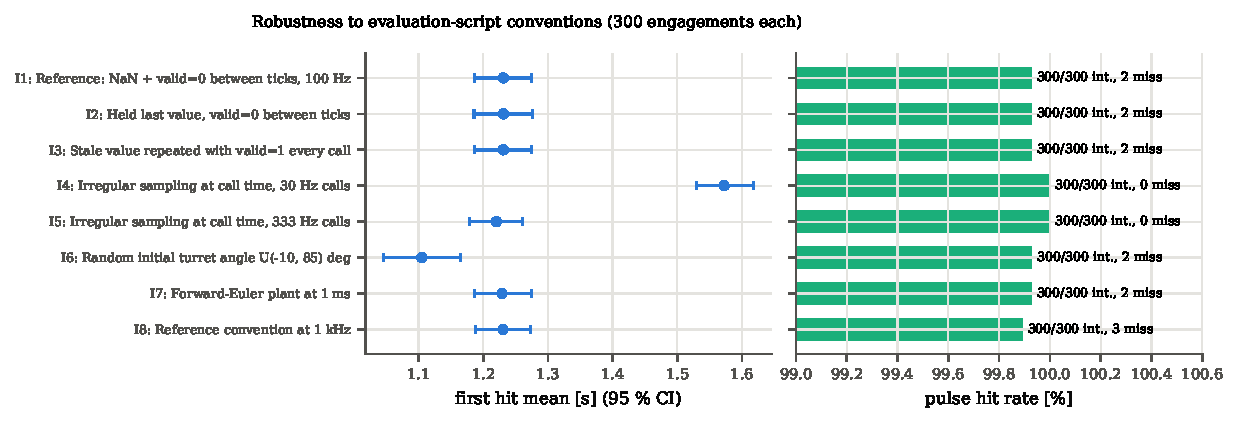
\includegraphics[width=\textwidth]{interface_robustness.pdf}
\caption{Frozen design under eight evaluation-script conventions (300 engagements each, identical seeds): mean first-hit time with 95\% CI, and pulse hit rate.}
\label{fig:interface}
\end{figure}

\begin{table}[H]
\centering\footnotesize
\caption{Robustness to evaluation-script conventions. $\Delta$ is paired against I1 (Wilcoxon $p$).}
\label{tab:interface}
\begin{tabularx}{\textwidth}{@{}lXcccc@{}}
\toprule
ID & Convention & Intercepted & Pulse hit rate (misses) & First hit mean / max [s] & $\Delta$ first hit [s], $p$\\
\midrule
I1 & reference, 100\,Hz & 300/300 & 99.93\% (2) & 1.231 / 2.05 & --\\
I2 & held value, \texttt{valid}=0 & 300/300 & 99.93\% (2) & 1.231 / 2.05 & 0, 1\\
I3 & stale value repeated, \texttt{valid}=1 & 300/300 & 99.93\% (2) & 1.231 / 2.05 & 0, 1\\
I4 & irregular sampling, 30\,Hz & 300/300 & 100.00\% (0) & 1.572 / 2.30 & $+0.341$, $7\times10^{-45}$\\
I5 & irregular sampling, 333\,Hz & 300/300 & 100.00\% (0) & 1.220 / 1.97 & $-0.011$, $10^{-25}$\\
I6 & random initial angle $-10^\circ$..$85^\circ$ & 300/300 & 99.93\% (2) & 1.105 / 2.80 & $-0.126$, $3\times10^{-4}$\\
I7 & forward-Euler plant, 1\,ms & 300/300 & 99.93\% (2) & 1.229 / 2.05 & $-0.002$, 0.99\\
I8 & reference, 1\,kHz & 300/300 & 99.89\% (3) & 1.231 / 1.96 & 0, --\\
\bottomrule
\end{tabularx}
\end{table}

\obs{
\begin{itemize}
\item \textbf{All 2\,400 engagements were intercepted} under every convention.
\item \textbf{Held or stale measurements are harmless.} I2 and I3 are bit-for-bit identical to I1, so the duplicate-measurement guard and the reliance on \texttt{meas\_valid} work. A script that keeps re-asserting \texttt{meas\_valid}=1 with an old sample, even through a blackout, cannot corrupt the track.
\item \textbf{Irregular radar timing is handled.} With samples taken whenever 50\,ms have elapsed, at call steps that do not divide 50\,ms (I4, I5), there were no misses at all. At 30\,Hz interception is 0.34\,s later, an effect of the coarse call rate (as in Section~8), not of the irregular timing. At 333\,Hz it matches the reference.
\item \textbf{Any initial turret angle works.} With the turret starting anywhere in $[-10^\circ,85^\circ]$ (I6), the worst first hit was 2.80\,s, consistent with the slew model of Section~\ref{sec:final}. The higher pointing RMS of this variant comes from 11 runs that started at $76^\circ$--$85^\circ$, whose long downward slews were still under way past the 2\,s mark where RMS starts counting.
\item \textbf{Plant integration and rate.} Forward-Euler at 1\,ms (I7) and a 1\,kHz call rate (I8) change nothing material.
\end{itemize}}
\takeaway{The design does not depend on our harness's conventions, so the unseen evaluation script should reproduce the performance reported here (supports H6).}
